\chapter{Desenvolvimento do sistema}
\label{cap:implementacao}
\begingroup
\setlength{\emergencystretch}{1.5em}
% Agrupar figuras com espaçamento fixo, sem grandes vazios entre elas.
\makeatletter
\setlength{\@fptop}{0pt}
\setlength{\@fpsep}{14pt}
\setlength{\@fpbot}{0pt plus 1fil}
\makeatother
\newcommand{\capfig}[4]{%
\begin{figure}[htbp]
\centering
\includegraphics[width=0.98\textwidth,height=#4\textheight,keepaspectratio]{Diagramas/plantuml/#1.png}
\caption{#2}\label{#3}
\fonte{Elaborado pelo autor (2026).}
\end{figure}
}
\section{Visão geral do sistema}
\label{sec:visao-sistema}
O sistema consiste em uma aplicação experimental para receber e armazenar registros de auditoria, acompanhada de um ambiente de avaliação das formas de comunicação. Um registro descreve um fato ocorrido, sua origem, a entidade envolvida e o ator responsável. O processamento compreende validação, serialização determinística, cálculo de SHA-256 e persistência com unicidade por identificador. O sistema não executa a operação de negócio que originou o fato, como alterar um cadastro: apenas recebe sua representação.

O público-alvo compreende pesquisadores e estudantes que reproduzam os ensaios e profissionais que analisem os custos de comunicação síncrona e assíncrona. A aplicação cliente envia eventos; o pesquisador configura o ambiente e interpreta as evidências. Não se prevê, neste escopo, um produto corporativo de auditoria, gerenciamento de usuários, edição de registros persistidos ou integração com dados pessoais reais.

Na variante síncrona, a API HTTP valida o evento e solicita ao repositório sua persistência antes de responder. Na variante assíncrona, outra API valida o mesmo contrato e encaminha a mensagem ao produtor Kafka. Um consumidor recebe as mensagens do tópico e utiliza o mesmo processamento e repositório. PostgreSQL mantém os registros; Kafka intermedeia o fluxo assíncrono. O monitoramento e os cenários de carga constituem uma camada experimental de geração, coleta e análise, separada da função de registro.

As funcionalidades implementadas incluem recebimento HTTP, validação, hash determinístico, persistência idempotente, confirmação individual de publicação, consumo, retry limitado, DLQ, confirmação de offsets, consultas de prontidão e de registro e documentação interativa das APIs para testes manuais. A geração de carga e a consolidação quantitativa ainda precisam ser adaptadas e validadas para esta implementação Java. Os quatro wireframes descrevem a interface de operação proposta; a comparação científica definitiva depende do protocolo e das repetições previstos no Capítulo~\ref{cap:metodo}. A Figura~\ref{fig:visao-geral} resume os dois caminhos operacionais implementados.

\begin{figure}[htbp]
\centering
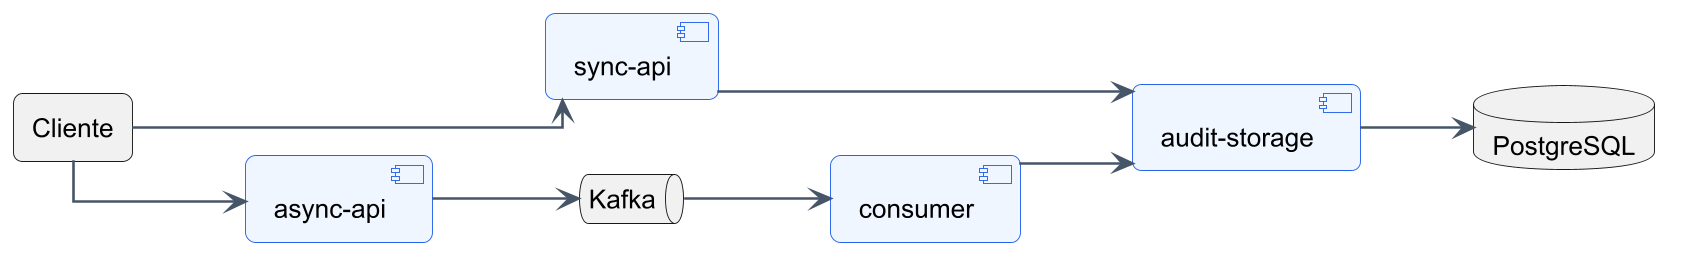
\includegraphics[width=0.95\textwidth,height=0.43\textheight,keepaspectratio]{Diagramas/plantuml/visao-geral.png}
\caption{Visão geral dos caminhos síncrono e assíncrono em Java}
\label{fig:visao-geral}
\fonte{Elaborado pelo autor (2026).}
\end{figure}

Nesta documentação, \textbf{implementado} indica que existe código para o comportamento descrito; as verificações disponíveis e seu alcance são apresentados na Seção~\ref{sec:validacao-funcional}. \textbf{Parcial} indica cobertura incompleta do requisito. \textbf{Planejado} identifica um componente ou procedimento ainda não implementado. Uma funcionalidade aprovada em teste não implica validação da hipótese científica.

A resposta \texttt{202 Accepted} sucede o ACK do broker e não significa que o registro já exista no PostgreSQL. Falhas de entrega podem produzir resultado incerto, enquanto falhas de consumo podem resultar em retry ou DLQ. A presença de uma mensagem na DLQ permite inspeção, mas não equivale a processamento concluído. O broker único limita a avaliação à topologia local, sem garantia de alta disponibilidade de cluster.

\textbf{Síntese.} As duas rotas executam o mesmo processamento e diferem na comunicação e nas condições de confirmação. O estado de cada requisito é vinculado ao código e às evidências, preservando a distinção entre validação funcional e comparação experimental.

\FloatBarrier
\section{Levantamento e especificação de requisitos}
\label{sec:requisitos}
Os identificadores RF01 a RF10 são preservados para manter a rastreabilidade com a documentação anterior. RF11 a RF15 tornam explícitas as funcionalidades de avaliação e interface previstas; RF16 e RF17 detalham tratamento de falhas e consulta por UUID. A prioridade \textbf{essencial} designa uma condição necessária ao núcleo ou à validade experimental; \textbf{desejável} designa uma facilidade de uso. A Tabela~\ref{tab:rf} distingue código Java existente de instrumentos planejados; o alcance dos testes está na Seção~\ref{sec:validacao-funcional}.

\subsection{Requisitos funcionais}
{\small
\begin{longtable}{>{\raggedright\arraybackslash}p{0.17\textwidth}>{\raggedright\arraybackslash}p{0.32\textwidth}>{\raggedright\arraybackslash}p{0.42\textwidth}}
\caption{Requisitos funcionais e critérios de aceitação}\label{tab:rf}\\
\hline
ID e estado & Descrição, prioridade e justificativa & Critério verificável de aceitação\\ \hline
\endfirsthead
\hline ID e estado & Descrição, prioridade e justificativa & Critério verificável de aceitação\\ \hline
\endhead
RF01\newline Implementado & Receber evento em \texttt{POST /audit}. Essencial: entrada equivalente nas variantes. & As duas APIs aceitam o mesmo JSON e retornam o UUID em respostas de sucesso.\\ \hline
RF02\newline Implementado & Validar contrato. Essencial: impedir dados estruturalmente inválidos. & UUID e data informados devem ser válidos; textos respeitam os limites do dicionário; entrada inválida retorna 422, sem processamento posterior.\\ \hline
RF03\newline Implementado & Concluir registro síncrono antes da resposta. Essencial: definir a semântica síncrona. & Resposta 201 ocorre somente após commit ou identificação de duplicata idêntica; status distingue \texttt{persisted} de \texttt{duplicate}.\\ \hline
RF04\newline Implementado & Encaminhar evento ao Kafka. Essencial: viabilizar processamento desacoplado. & Evento preserva UUID e conteúdo; chave é \texttt{entity\_id}. 202 somente após ACK individual do broker com tópico, partição e offset no log. Timeout de entrega retorna 503 com resultado incerto.\\ \hline
RF05\newline Implementado & Consumir mensagens. Essencial: concluir a rota assíncrona. & Mensagem válida do tópico configurado é desserializada, validada e encaminhada ao mesmo repositório da variante síncrona.\\ \hline
RF06\newline Implementado & Gerar hash determinístico. Essencial: detectar conteúdo divergente. & O mesmo evento completo gera o mesmo SHA-256 hexadecimal de 64 caracteres; a ordenação de chaves não altera a representação serializada.\\ \hline
RF07\newline Implementado & Persistir registro. Essencial: manter efeito observável. & Linha contém os campos de \texttt{AuditEvent} e \texttt{content\_hash}; \texttt{event\_id} é chave primária.\\ \hline
RF08\newline Implementado & Reconhecer reentrega idêntica. Essencial: evitar efeito duplicado. & Duas submissões com UUID e conteúdo iguais mantêm uma linha e retornam status de duplicata na segunda; conteúdo divergente não substitui o original.\\ \hline
RF09\newline Implementado & Confirmar offset após persistência. Essencial: reduzir risco de perda por confirmação antecipada. & Commit automático desativado; confirmar origem somente após persistência idempotente ou ACK da DLQ. Falha de confirmação mantém possibilidade de reentrega.\\ \hline
RF10\newline Implementado & Expor \texttt{GET /health}. Essencial: verificar resposta da API. & \texttt{/health} verifica PostgreSQL na API síncrona e metadados do tópico na assíncrona; retorna 200 ou 503. \texttt{/live} verifica apenas a resposta do processo.\\ \hline
RF11\newline Planejado & Coletar métricas por execução. Essencial: responder à pergunta experimental. & Um futuro coletor deverá produzir arquivos conciliáveis por UUID e execução, com aceitação, conclusão, throughput, erros e recursos, incluindo unidade e janela. Os logs Java isolados não satisfazem esse critério.\\ \hline
RF12\newline Parcial & Executar cenários de carga e falha. Essencial: controle experimental. & Há um \textit{smoke} de interrupção do banco na CI. O executor definitivo ainda deverá registrar taxa, duração, semente, variante, falha e configuração em manifesto reproduzível.\\ \hline
RF13\newline Parcial & Acompanhar recuperação. Essencial: avaliar comportamento após falhas. & O \textit{smoke} verifica retomada da saúde do banco, mas ainda falta registrar backlog, drenagem e conciliação dos eventos aceitos e persistidos.\\ \hline
RF14\newline Planejado & Consultar indicadores e comparar variantes. Desejável: facilitar inspeção. & Um relatório futuro deverá separar latência HTTP de conclusão e sinalizar ausência de dados. Não há interface ou normalizador comparativo Java implementado.\\ \hline
RF15\newline Planejado & Disponibilizar formulário de envio. Desejável: facilitar demonstração. & O wireframe preserva UUID e instante e distingue variantes. A interface dedicada e documentação interativa de API não integram a implementação Java atual.\\ \hline
RF16\newline Implementado & Tratar falhas e quarentena. Essencial: evitar perda por avanço prematuro. & Aplicar retry limitado com backoff; publicar erro terminal na DLQ e aguardar ACK antes de confirmar a origem.\\ \hline
RF17\newline Implementado & Consultar registro por UUID. Essencial: verificar efeito persistido. & A API síncrona retorna hash e timestamp da linha; 404 indica ausência observada e 503 indica consulta indisponível.\\ \hline
\end{longtable}
\noindent{\footnotesize Fonte: Elaborado pelo autor (2026).}\par
}

\subsection{Requisitos não funcionais}
A Tabela~\ref{tab:rnf} relaciona propriedades de qualidade, critérios verificáveis e justificativas.
Desempenho não é definido por um código HTTP: 201 e 202 não são limites de tempo. Não se impõe, antes do piloto, que a alternativa assíncrona seja mais rápida. Os critérios de medição e as condições de comparação substituem expressões não verificáveis como \textit{tempo reduzido}.

{\small
\begin{longtable}{>{\raggedright\arraybackslash}p{0.12\textwidth}>{\raggedright\arraybackslash}p{0.24\textwidth}>{\raggedright\arraybackslash}p{0.55\textwidth}}
\caption{Requisitos não funcionais}\label{tab:rnf}\\
\hline ID & Categoria e prioridade & Critério e justificativa\\ \hline
\endfirsthead
\hline ID & Categoria e prioridade & Critério e justificativa\\ \hline
\endhead
RNF01 & Equivalência; essencial & Utilizar DTO, serialização e repositório comuns; comparar o mesmo conjunto de eventos com a mesma configuração de persistência. Evita atribuir diferenças funcionais à comunicação.\\ \hline
RNF02 & Reprodutibilidade; essencial & Registrar imagens, dependências, commit, recursos, scripts e parâmetros. O Compose explicita limites de desenvolvimento; manifesto e checksums da coleta definitiva ainda precisam ser implementados e validados.\\ \hline
RNF03 & Segurança; essencial & Usar dados sintéticos sem segredos; executar em ambiente isolado. O protótipo não possui autenticação nem é autorizado para exposição pública ou dados pessoais reais.\\ \hline
RNF04 & Portabilidade; essencial & Descrever build e inicialização com Docker Compose, além dos pré-requisitos. Versões de bibliotecas são fixadas; tags de imagens deverão ter digest registrado na coleta.\\ \hline
RNF05 & Integridade e correlação; essencial & Preservar UUID e instante de origem nos reenvios; manter hash e restrição de unicidade. Conflitos devem ser distinguíveis de duplicatas legítimas nos registros de diagnóstico.\\ \hline
RNF06 & Desempenho; essencial & Medir latência de aceitação e de conclusão separadamente, p50/p95/p99, throughput persistido e taxa oferecida; definir tolerâncias de carga no piloto, conforme o Capítulo~\ref{cap:metodo}.\\ \hline
RNF07 & Resiliência; essencial & Após falha controlada e retomada, conciliar os UUIDs dentro da janela de drenagem; zero linhas duplicadas. Eventos na DLQ exigem tratamento posterior e não retornam automaticamente ao banco.\\ \hline
RNF08 & Observabilidade; essencial & Registrar execução, UUID, componente, etapa, instante e resultado; coletar recursos com intervalo fixado. Os marcos JSON já existem; coletores, completude e resolução temporal ainda precisam de validação para cada execução definitiva.\\ \hline
RNF09 & Escalabilidade; desejável & Registrar partições e número de consumidores em cada configuração. Não inferir escalabilidade horizontal a partir de uma execução em broker único.\\ \hline
RNF10 & Usabilidade experimental; desejável & Identificar a variante e o estado dos dados em cada tela; oferecer mensagens legíveis e unidades. Wireframes não equivalem a um painel implementado.\\ \hline
\end{longtable}
\noindent{\footnotesize Fonte: Elaborado pelo autor (2026).}\par
}

\subsection{Regras de negócio}
Neste contexto, regras de negócio são invariantes do processamento de auditoria e do contrato experimental, e não políticas de um sistema comercial.

\begin{description}
\item[RN01 --- Identidade.] Todo evento processado possui UUID. O DTO gera UUID se omitido; nos ensaios, o gerador deverá fornecê-lo antes do envio e preservá-lo nas novas tentativas. Novo UUID significa novo evento.
\item[RN02 --- Validação.] Tipo do evento, tipo e ID da entidade, ator e origem são obrigatórios e respeitam os limites do DTO. UUID, instante e payload possuem valores padrão quando omitidos. A obrigatoriedade no banco não significa obrigatoriedade de envio desses três campos na API. Na mensagem Kafka, identidade e instante devem estar explícitos: o consumidor rejeita sua ausência para que uma reentrega não gere outro evento.
\item[RN03 --- Hash.] O SHA-256 abrange todos os campos do evento validado, incluindo UUID e instante. JSON usa chaves ordenadas e separadores compactos. A regra é determinística no contexto da implementação; não se declara conformidade com um padrão externo de canonicalização.
\item[RN04 --- Idempotência.] Mesmo UUID e mesmo hash preservam a linha original e produzem status \texttt{duplicate}. O cliente deve reenviar o mesmo instante; gerar outra data pode tornar o conteúdo divergente.
\item[RN05 --- Conflito.] Mesmo UUID e hash diferente não podem sobrescrever a linha. A API síncrona retorna 409 com motivo \texttt{event\_id\_content\_conflict}. No consumidor, o conflito é encaminhado à DLQ sem alterar a linha original.
\item[RN06 --- Aceitação assíncrona.] O 202 não confirma persistência em PostgreSQL. Confirma publicação segundo \texttt{acks=all} e a topologia configurada. Se o ACK não chegar no prazo, a resposta 503 informa resultado incerto; o cliente deve conciliar e preservar o evento completo em eventual reenvio.
\item[RN07 --- Offset e falha.] O offset de origem é confirmado após inserção, reconhecimento idempotente ou ACK da DLQ. Falhas de persistência recebem tentativas limitadas com backoff. Se DLQ ou commit de offset não forem confirmados, a sessão é retomada sem avançar além da origem não resolvida.
\item[RN08 --- Confirmação síncrona.] A API retorna 201 após persistência ou reconhecimento de reentrega, distinguindo-os pelo campo status. Em falha de persistência não deve declarar sucesso.
\item[RN09 --- Particionamento.] A chave enviada ao produtor é \texttt{entity\_id}. A ordem relativa depende da manutenção da chave, do particionamento e da sequência produzida; não se promete ordenação global entre partições.
\item[RN10 --- Evidência experimental.] As métricas definitivas deverão identificar execução, variante, unidade e janela. Eventos gerados, aceitos e persistidos são conjuntos distintos. O marco pós-commit comum define conclusão; instante de ocorrência e timestamp de inserção não o substituem.
\item[RN11 --- Quarentena.] Mensagens inválidas, conflitos e tentativas esgotadas são retidos na DLQ. A chave de origem usa tópico, partição e offset. Se a DLQ for confirmada e o commit de origem falhar, podem existir cópias na DLQ; a conciliação futura deverá usar essa chave. Não há replay automático de mensagens em quarentena.
\end{description}
\textbf{Síntese.} Os requisitos indicam o comportamento esperado, o critério de verificação e o estado de implementação. As regras tornam explícitos os limites do aceite assíncrono, da identidade do evento e da recuperação.

\section{Modelagem UML}
\label{sec:uml}
As vistas representam o contrato, as responsabilidades e os caminhos de execução. A fronteira operacional é a implementação Java, com duas APIs Spring Boot e um consumidor independente; Kafka e PostgreSQL são sistemas externos de suporte. Na visão de implantação, esses serviços integram a infraestrutura do ambiente experimental. As bibliotecas Maven compartilhadas não são atores nem processos independentes.

\subsection{Diagrama de casos de uso}
A aplicação cliente inicia UC01 e UC02; Kafka fornece mensagens a UC03; o pesquisador consulta prontidão e registros em UC04 e UC07. A Figura~\ref{fig:casos-uso} apresenta essas interações. A Figura~\ref{fig:casos-exp} reúne os casos planejados de avaliação quantitativa, cujo executor ainda não integra o projeto Java.

\capfig{casos-de-uso}{Casos de uso da aplicação operacional}{fig:casos-uso}{0.44}
\capfig{casos-experimento}{Casos de uso da camada de avaliação}{fig:casos-exp}{0.25}

\subsubsection{UC01 --- Registrar auditoria sincronamente}
\textbf{Objetivo e atores:} persistir evento antes da resposta; aplicação cliente e PostgreSQL.
\textbf{Pré-condições:} API inicializada e banco acessível.
\textbf{Ativação:} \texttt{POST /audit}.
\textbf{Pós-condição:} linha inserida ou reentrega idêntica reconhecida.
\textbf{Regras:} RN01--RN05 e RN08.
\begin{enumerate}
\item A aplicação envia o evento à API síncrona.
\item O contrato é validado e recebe os valores padrão permitidos.
\item O repositório calcula a representação determinística e o SHA-256.
\item Executa \texttt{INSERT ON CONFLICT DO NOTHING}, verificando o resultado.
\item A transação é concluída; o marco pós-commit é registrado.
\item A API retorna 201, UUID, hash, status e timestamp de inserção.
\end{enumerate}
\textbf{A1 --- Reentrega:} quando o UUID já existe, uma nova consulta na mesma transação em \texttt{READ COMMITTED} obtém a linha. Hash igual produz \texttt{duplicate}; nenhuma nova linha é criada.
\textbf{E1 --- Contrato inválido:} retorna 422 antes de chamar o repositório.
\textbf{E2 --- Conflito:} hash diferente provoca rollback e resposta 409 com \texttt{event\_id\_content\_conflict}, preservando a linha original.
\textbf{E3 --- Banco indisponível:} retorna 503 com \texttt{database\_unavailable}. Uma falha durante o commit pode deixar o resultado incerto; consulta e reenvio devem preservar o evento completo.

\subsubsection{UC02 --- Aceitar auditoria assincronamente}
\textbf{Objetivo e atores:} confirmar publicação sem aguardar persistência; aplicação cliente e Kafka.
\textbf{Pré-condição:} API e publicador inicializados.
\textbf{Ativação:} \texttt{POST /audit} na API assíncrona.
\textbf{Pós-condição:} publicação confirmada individualmente pelo broker.
\textbf{Regras:} RN01, RN02, RN06 e RN09.
\begin{enumerate}
\item A API valida o mesmo contrato da variante síncrona.
\item Serializa os campos completos e usa \texttt{entity\_id} como chave.
\item O publicador chama \texttt{send(...).get(...)} e aguarda a confirmação individual dentro do prazo.
\item Registra o ACK, incluindo tópico, partição e offset, e retorna 202.
\end{enumerate}
\textbf{A1 --- Reenvio:} a API não consulta duplicidade; o consumidor e o banco reconhecem eventos idênticos.
\textbf{E1 --- Contrato inválido:} retorna 422.
\textbf{E2 --- Buffer do produtor cheio:} retorna 503 com \texttt{acceptance=rejected}.
\textbf{E3 --- Timeout ou erro de confirmação:} retorna 503 com \texttt{acceptance=unknown}. A mensagem pode ter sido entregue; a resposta não autoriza assumir perda.
\textbf{Limite:} ACK de publicação e persistência são pós-condições distintas. O consumidor pode processar a mensagem antes ou depois de o cliente receber a resposta.

\subsubsection{UC03 --- Consumir e persistir evento}
\textbf{Objetivo e atores:} processar ou reter uma falha identificável; Kafka e PostgreSQL.
\textbf{Pré-condições:} consumidor inscrito no tópico e configuração de retry válida.
\textbf{Ativação:} mensagem retornada por \texttt{poll}.
\textbf{Pós-condição:} persistência idempotente ou retenção confirmada na DLQ, seguida da confirmação da posição de origem.
\textbf{Regras:} RN03--RN05, RN07, RN09 e RN11.
\begin{enumerate}
\item O consumidor recebe a mensagem e recupera o identificador da execução.
\item Valida JSON, contrato e presença explícita de UUID e instante.
\item Registra a tentativa e chama o repositório comum.
\item Depois da transação ou reconhecimento de duplicata, registra o resultado.
\item Confirma o offset de origem de forma síncrona e retorna à espera.
\end{enumerate}
\textbf{A1 --- Reentrega idêntica:} preserva a linha e confirma a posição após reconhecimento de duplicata.
\textbf{A2 --- Falha transitória:} repete a persistência até o limite configurado, com backoff exponencial limitado e registro das tentativas.
\textbf{E1 --- Mensagem inválida, conflito ou tentativas esgotadas:} publica envelope na DLQ com identidade da origem, motivo e conteúdo original, aguarda ACK e então confirma a origem.
\textbf{E2 --- DLQ não confirmada:} retoma a sessão sem confirmar a mensagem de origem. Mensagens posteriores não justificam avançar sua posição.
\textbf{E3 --- Falha de commit de offset:} retoma a sessão; a persistência ou a publicação em DLQ já pode ter ocorrido. A reentrega é tratada por UUID no banco ou pela identidade da origem na conciliação da DLQ.
\textbf{E4 --- Dependência indisponível:} o laço externo aguarda e reinicia a sessão; a política de restart do Compose cobre encerramento do processo. Mensagens já retidas na DLQ exigem inspeção e não retornam automaticamente ao fluxo principal.

\subsubsection{UC04 --- Consultar prontidão}
\textbf{Ator:} pesquisador.
\textbf{Ativação:} \texttt{GET /health}.
\textbf{Pré-condição:} processo HTTP iniciado.
\textbf{Fluxo principal:} verificar acesso ao esquema PostgreSQL na API síncrona ou existência e liderança das partições do tópico na API assíncrona; retornar 200 com \texttt{ready}.
\textbf{Alternativa:} \texttt{GET /live} retorna \texttt{alive} para verificar apenas a resposta do processo.
\textbf{Exceção:} dependência sem prontidão produz 503; processo parado causa falha de conexão.
\textbf{Pós-condição:} resultado de uma verificação pontual, sem garantia de disponibilidade futura ou de conclusão de todos os eventos. Relaciona-se a RF10.

\subsubsection{UC05 --- Executar cenário de avaliação (planejado)}
\textbf{Ator:} pesquisador.
\textbf{Pré-condições:} ambiente isolado preparado, dados sintéticos e configuração identificada; protocolo congelado para coleta definitiva.
\textbf{Ativação prevista:} comando do executor e seleção do perfil.
\textbf{Fluxo previsto:} criar diretório exclusivo; registrar manifesto; preparar eventos; executar aquecimento e carga; coletar logs, recursos e offsets; interromper o PostgreSQL em C4; registrar a retomada; aguardar drenagem; consolidar arquivos.
\textbf{Alternativas:} teste dos instrumentos ou execução conforme protocolo definitivo.
\textbf{Exceção prevista:} configuração incompleta ou falha de coleta deve ser registrada; validação funcional não vira resultado definitivo.
\textbf{Pós-condição esperada:} artefatos verificáveis da execução, com indicação de completude. O projeto Java atual contém apenas \textit{smokes} de CI, sem esse executor. Relaciona-se a RF12, RF13 e RN10.

\subsubsection{UC06 --- Consolidar e consultar indicadores (planejado)}
\textbf{Ator:} pesquisador.
\textbf{Pré-condição:} arquivos brutos de execução disponíveis.
\textbf{Ativação prevista:} execução de um normalizador ainda não adaptado ao Java.
\textbf{Fluxo previsto:} verificar arquivos; correlacionar UUIDs; separar fases; calcular métricas e unidades; registrar inconsistências; produzir tabelas e relatório.
\textbf{Alternativa:} inspecionar lag, reentregas, retry, DLQ e recuperação.
\textbf{Exceção:} ausência de instrumentação é sinalizada e não substituída por medição zero.
\textbf{Pós-condição esperada:} indicadores rastreáveis aos dados brutos. A interface dedicada dos wireframes permanece proposta. Relaciona-se a RF11, RF14 e RN10.

\subsubsection{UC07 --- Consultar registro por UUID}
\textbf{Ator:} pesquisador ou aplicação cliente.
\textbf{Pré-condições:} API síncrona e banco acessíveis.
\textbf{Ativação:} \texttt{GET /audit/\{event\_id\}}.
\textbf{Fluxo principal:} validar UUID, consultar a projeção da linha e retornar 200 com hash e timestamp.
\textbf{Alternativa:} após reenvio, conferir a preservação do hash.
\textbf{Exceções:} UUID inválido retorna 422; linha não localizada, 404; banco indisponível, 503.
\textbf{Pós-condição:} existência ou ausência observada naquele instante; 404 durante processamento assíncrono não prova perda. Relaciona-se a RF17 e RN04.

\subsection{Diagramas de atividades}
A Figura~\ref{fig:atividade-sync} representa a inserção síncrona e as decisões de duplicidade e conflito. As Figuras~\ref{fig:atividade-async} e~\ref{fig:atividade-consumidor} separam o aceite da API produtora e o processamento do consumidor. Os dois processos assíncronos não dependem da ordem em que a resposta HTTP chega ao cliente.

\capfig{atividade-sincrona}{Atividade síncrona: transação, duplicidade e conflito}{fig:atividade-sync}{0.62}
\capfig{atividade-assincrona}{Atividade da API produtora e confirmação de publicação}{fig:atividade-async}{0.59}
\capfig{atividade-consumidor}{Atividade do consumidor, retry e confirmação da origem}{fig:atividade-consumidor}{0.75}

A atividade de persistência com retry corresponde ao laço limitado de UC03. O caminho de quarentena inclui a espera pelo ACK da DLQ. Um término da iteração não significa encerramento do serviço: o laço externo mantém a espera ou a reconexão, conforme indicado nas ações.

\FloatBarrier
\subsection{Diagramas de classes}
A Figura~\ref{fig:classes-dados} apresenta os \textit{records} do contrato e o repositório JDBC. A Figura~\ref{fig:classes} mostra as classes de entrada e processamento dos três módulos executáveis, além das dependências compartilhadas. Nenhuma herança ORM é representada porque o projeto Java usa Spring JDBC e uma migração SQL.

\capfig{classes-dados}{Classes de contrato e persistência}{fig:classes-dados}{0.46}
\capfig{classes}{Classes de aplicação e processamento Java}{fig:classes}{0.45}

A notação \(+\) indica membros públicos. A validação pertence ao contrato \texttt{AuditEvent}. A serialização e o hash ficam na \texttt{CanonicalEventCodec}; a transação, na \texttt{AuditRepository}; e os marcos, na \texttt{MilestoneLog}. O broker é infraestrutura, não classe de domínio. O \texttt{AuditMessageProcessor} chama \texttt{commitSync} sobre o consumidor Kafka depois da persistência ou do ACK da DLQ.

\FloatBarrier
\subsection{Diagramas complementares}
As Figuras~\ref{fig:seq-sync} e~\ref{fig:seq-async} detalham a ordem entre transação, resposta, ACK e confirmação de posição. A Figura~\ref{fig:componentes} sintetiza as dependências entre os módulos Maven; o caminho de publicação na DLQ pelo consumidor é detalhado na atividade, na sequência e na arquitetura assíncronas para manter esta vista legível. As Figuras~\ref{fig:arq-sync} e~\ref{fig:arq-async} distinguem os fluxos arquiteturais e a participação da DLQ.

\capfig{sequencia-sincrona}{Sequência síncrona com inserção idempotente}{fig:seq-sync}{0.62}
\capfig{sequencia-assincrona}{Sequência assíncrona com ACK e tratamento de falhas}{fig:seq-async}{0.61}
\capfig{componentes}{Dependências entre os cinco módulos Maven}{fig:componentes}{0.44}
\capfig{arquitetura-sincrona}{Arquitetura da variante síncrona}{fig:arq-sync}{0.38}
\capfig{arquitetura-assincrona}{Arquitetura da variante assíncrona e DLQ}{fig:arq-async}{0.43}

\subsubsection{Diagrama de implantação}
A Figura~\ref{fig:implantacao} localiza os cinco serviços permanentes na rede Docker Compose e separa o cliente de carga, executado pelo pesquisador, dos processos de aplicação. Os serviços \texttt{kafka-init} e \texttt{kafka-volume-init} são transitórios e, por isso, aparecem na anotação do diagrama, não como processos permanentes. As portas publicadas estão restritas ao \textit{loopback} do host. Os volumes nomeados conservam os dados do PostgreSQL e os logs do Kafka entre reinícios de contêiner. Esta é uma implantação experimental com um broker, uma partição por tópico e um banco; não representa alta disponibilidade.

\capfig{implantacao}{Implantação real do protótipo no Docker Compose}{fig:implantacao}{0.48}

\FloatBarrier
\subsection{Rastreabilidade entre requisitos, regras e UML}
A Tabela~\ref{tab:rastreabilidade} relaciona cada requisito funcional às regras e aos elementos que o representam. Os elementos planejados não indicam código já existente. A cobertura funcional verificada é delimitada na Seção~\ref{sec:validacao-funcional}.
{\small
\begin{longtable}{p{0.20\textwidth}p{0.20\textwidth}p{0.51\textwidth}}
\caption{Rastreabilidade funcional e comportamental}\label{tab:rastreabilidade}\\
\hline Requisitos & Regras & Casos e elementos de modelagem\\ \hline
\endfirsthead
\hline Requisitos & Regras & Casos e elementos de modelagem\\ \hline
\endhead
RF01, RF02 & RN01, RN02 & UC01, UC02; AuditEvent e validação dos dois fluxos.\\ \hline
RF03, RF06, RF07 & RN03, RN08 & UC01; atividade e sequência síncronas; CanonicalEventCodec e AuditRepository.\\ \hline
RF04 & RN06, RN09 & UC02; KafkaPublisher; ACK na atividade e sequência assíncronas.\\ \hline
RF05, RF09, RF16 & RN07, RN11 & UC03; retry, DLQ e confirmação de origem; atividade do consumidor.\\ \hline
RF08 & RN04, RN05 & UC01 e UC03; decisões de hash e unicidade; tabela audit\_records.\\ \hline
RF10 & RN10 & UC04; prontidão e vivacidade das APIs.\\ \hline
RF11, RF14 & RN10 & UC06 planejado; normalizador e wireframes de métricas/comparação.\\ \hline
RF12, RF13 & RN07, RN10 & UC05 planejado; protocolo e acompanhamento de backlog ainda incompletos.\\ \hline
RF15 & RN01, RN02, RN06 & UC01 e UC02; wireframe de envio com identidade preservada.\\ \hline
RF17 & RN04, RN05 & UC07; consulta por UUID no repositório.\\ \hline
\end{longtable}
\noindent{\footnotesize Fonte: Elaborado pelo autor (2026).}\par
}
\textbf{Síntese.} Os casos de uso descrevem objetivos e exceções; atividades e sequências mostram as decisões; classes e componentes localizam suas responsabilidades. As condições da coleta definitiva permanecem ligadas ao protocolo metodológico.

\section{Modelagem de banco de dados}
\label{sec:banco}
A modelagem distingue o esquema operacional da extensão relacional proposta. O banco da implementação Java possui somente a tabela \texttt{audit\_records}, criada pela migração Flyway \texttt{V1\_\_create\_audit\_records.sql}. O acesso usa Spring JDBC; não há mapeamento ORM nem rotina de adaptação de linhas históricas da versão Python. Marcos de execução são emitidos nos logs da aplicação, fora do banco operacional. A coleta estruturada de métricas e tentativas para o experimento ainda será desenvolvida. As tabelas adicionais desta seção permanecem propostas opcionais.

\subsection{Modelo conceitual (MER)}
A Figura~\ref{fig:mer-atual} apresenta o núcleo e a Figura~\ref{fig:mer-proposto} apresenta a extensão proposta. No núcleo atual, a entidade \textit{Registro de auditoria} representa o fato persistido e contém identificação, origem, instante, entidade, ator, conteúdo e hash. Não há relacionamento entre tabelas no esquema existente. O hash é atributo do registro, pois há exatamente um digest armazenado por linha; criar uma entidade \textit{EventHash} independente não acrescentaria informação necessária ao recorte e criaria uma sincronização adicional.

A extensão proposta introduz \textit{Log de processamento}, \textit{Tentativa de recuperação} e \textit{Amostra de métrica}. Um UUID pode aparecer em zero ou muitos logs, inclusive quando nenhuma linha de auditoria foi persistida. Cada log representa uma tentativa ou etapa observada. Um log pode originar zero ou muitas tentativas de recuperação; cada tentativa referencia um log. Métricas agregadas são associadas ao identificador da execução, e não obrigatoriamente a um único evento.

\capfig{mer-atual}{Modelo conceitual do núcleo existente}{fig:mer-atual}{0.25}
\capfig{mer-proposto}{Modelo conceitual da extensão de observabilidade proposta}{fig:mer-proposto}{0.40}

A associação entre registro e log é de correlação por UUID, não de existência obrigatória: um erro pode ocorrer antes da primeira inserção. Não se estabelece uma chave estrangeira obrigatória de log para \texttt{audit\_records}, pois isso impediria registrar justamente a falha de persistência. A tentativa de recuperação, por sua vez, referencia um log já existente. Essa distinção preserva a capacidade de registrar eventos rejeitados, falhas e reentregas sem pressupor sucesso.

\subsection{Modelo lógico}
No esquema atual, \texttt{audit\_records.event\_id} é chave primária; \texttt{entity\_id} possui o índice secundário \texttt{idx\_audit\_records\_entity\_id}; os atributos do evento e o hash são não nulos. A coluna \texttt{persisted\_at} é anulável no DDL, embora novas inserções recebam \texttt{clock\_timestamp()} por padrão. A Figura~\ref{fig:der-atual} representa somente a tabela implementada. Não existem chaves estrangeiras ou relacionamentos entre tabelas. A restrição de unicidade protege contra inserções concorrentes com o mesmo UUID. O hash é calculado na aplicação e armazenado como texto; não há restrição SQL de comprimento do digest.

\capfig{modelo-logico-atual}{Modelo lógico do banco implementado}{fig:der-atual}{0.38}

\subsection{Modelo físico implementado}
O arquivo \texttt{audit-storage/src/main/resources/db/migration/V1\_\_create\_audit\_records.sql} cria a tabela no PostgreSQL. Sua chave primária sobre \texttt{event\_id} é a única restrição de unicidade explícita. \texttt{entity\_id} recebe índice não único \texttt{idx\_audit\_records\_entity\_id}. Os nove campos obrigatórios são \texttt{event\_id}, \texttt{event\_type}, \texttt{entity\_type}, \texttt{entity\_id}, \texttt{actor\_id}, \texttt{source}, \texttt{occurred\_at}, \texttt{payload} e \texttt{content\_hash}. O décimo campo, \texttt{persisted\_at}, é anulável e possui \texttt{DEFAULT clock\_timestamp()}. Não existe chave estrangeira, gatilho, exclusão lógica ou tabela de usuários nesse esquema.

O Flyway aplica a migração V1 na inicialização da API síncrona e do consumidor sobre o banco novo desta versão. Não há migração automática do banco Python nem compatibilidade retroativa demonstrada. A garantia de idempotência combina a PK, o \texttt{INSERT ON CONFLICT DO NOTHING} e a comparação do \texttt{content\_hash} no \texttt{AuditRepository} após a tentativa de inserção. Portanto, o modelo físico deve ser entendido junto à regra implementada na aplicação, e não como uma restrição SQL de igualdade do conteúdo.

\subsection{Extensão lógica opcional}
A Figura~\ref{fig:der} apresenta, separadamente, a possível extensão de observabilidade. As entidades destacadas como \textit{propostas} não foram criadas pelo código e não integram o banco utilizado nos testes.

\capfig{modelo-logico}{Modelo lógico da extensão proposta, separado do esquema atual}{fig:der}{0.57}

Na extensão, \texttt{processing\_log.id}, \texttt{retry\_log.id} e \texttt{metrics.id} são chaves primárias propostas. \texttt{retry\_log.processing\_log\_id} referencia o log que motivou a tentativa. \texttt{run\_id} correlaciona os três conjuntos com o manifesto externo de execução. Não se cria uma tabela de execuções nesta proposta inicial; caso isso seja feito posteriormente, o manifesto poderá ser normalizado em uma entidade própria.

A unicidade proposta de \texttt{(run\_id, event\_id, component, attempt)} em logs identifica uma tentativa por componente. Índices por execução, UUID e instante apoiam conciliação. Status e unidades deverão ser validados pela camada de coleta. Migrações e consultas dessas tabelas são atividades futuras, não executadas para produzir este texto. A instrumentação deverá ser equivalente entre variantes e ter seu custo considerado na análise experimental.

\FloatBarrier
\subsection{Dicionário de dados}

\subsubsection{Tabela audit\_records --- existente}
A Tabela~\ref{tab:dic-audit} descreve o esquema efetivo. Os campos do evento e o hash são não nulos; \texttt{persisted\_at} admite nulo pelo DDL da migração Java. No recebimento HTTP, \texttt{event\_id}, \texttt{occurred\_at} e \texttt{payload} podem ser omitidos e recebem valores padrão.

{\small
\begin{longtable}{>{\raggedright\arraybackslash}p{0.23\textwidth}>{\raggedright\arraybackslash}p{0.22\textwidth}>{\raggedright\arraybackslash}p{0.46\textwidth}}
\caption{Dicionário do registro persistido}\label{tab:dic-audit}\\
\hline Campo & Tipo e tamanho & Obrigatoriedade, significado e validação\\ \hline
\endfirsthead
\hline Campo & Tipo e tamanho & Obrigatoriedade, significado e validação\\ \hline
\endhead
\texttt{event\_id} & UUID, 128 bits & PK; não nulo. UUID informado deve ser válido; uuid4 gerado se ausente. Deve ser preservado em reenvios experimentais.\\ \hline
\texttt{event\_type} & VARCHAR(100) & Não nulo; obrigatório na API, 1--100 caracteres. Tipo do fato observado; sem enumeração fechada implementada.\\ \hline
\texttt{entity\_type} & VARCHAR(100) & Não nulo; obrigatório, 1--100 caracteres. Tipo da entidade referida.\\ \hline
\texttt{entity\_id} & VARCHAR(200) & Não nulo; obrigatório, 1--200 caracteres; índice. Identificador da entidade e chave enviada ao Kafka.\\ \hline
\texttt{actor\_id} & VARCHAR(200) & Não nulo; obrigatório, 1--200 caracteres. Ator sintético relacionado ao fato.\\ \hline
\texttt{source} & VARCHAR(100) & Não nulo; obrigatório, 1--100 caracteres. Sistema ou componente de origem.\\ \hline
\texttt{occurred\_at} & TIMESTAMP WITH TIME ZONE & Não nulo. Instante de ocorrência; padrão UTC atual se omitido. Quando informado, o Java interpreta data ISO-8601 com offset. Não representa instante de commit.\\ \hline
\texttt{payload} & JSONB & Não nulo; objeto com padrão vazio. Sem limite de tamanho ou profundidade definido no DTO atual. Conteúdo contextual sintético.\\ \hline
\texttt{content\_hash} & TEXT & Não nulo. SHA-256 calculado, 64 caracteres hexadecimais; o tipo SQL não impõe esse comprimento. Inclui os campos completos do evento.\\ \hline
\texttt{persisted\_at} & TIMESTAMP WITH TIME ZONE & Anulável pelo DDL. Novas linhas recebem clock\_timestamp() durante INSERT. Não representa conclusão do commit.\\ \hline
\end{longtable}
\noindent{\footnotesize Fonte: Elaborado pelo autor (2026).}\par
}

\subsubsection{Tabela processing\_log --- proposta}
A Tabela~\ref{tab:dic-processing} descreve a proposta de uma tentativa por componente. Ela não substitui o evento original nem modifica sua identidade.

{\small
\begin{longtable}{>{\raggedright\arraybackslash}p{0.23\textwidth}>{\raggedright\arraybackslash}p{0.22\textwidth}>{\raggedright\arraybackslash}p{0.46\textwidth}}
\caption{Dicionário proposto dos logs de processamento}\label{tab:dic-processing}\\
\hline Campo & Tipo e tamanho & Obrigatoriedade e regra proposta\\ \hline
\endfirsthead
\hline Campo & Tipo e tamanho & Obrigatoriedade e regra proposta\\ \hline
\endhead
\texttt{id} & BIGINT identity & PK, obrigatório. Identifica o log.\\ \hline
\texttt{run\_id} & UUID & Obrigatório. Correlaciona com o manifesto de execução.\\ \hline
\texttt{event\_id} & UUID & Obrigatório para eventos identificáveis. Correlação, sem FK para o registro persistido. Erros sem UUID ficam no log técnico do coletor.\\ \hline
\texttt{component} & VARCHAR(30) & Obrigatório. Identifica API síncrona, API produtora ou consumidor.\\ \hline
\texttt{status} & VARCHAR(30) & Obrigatório. Vocabulário proposto: accepted, persisted, duplicate, rejected, failed ou conflict.\\ \hline
\texttt{attempt} & INTEGER & Obrigatório; maior ou igual a 1. Número da tentativa por evento e componente na execução.\\ \hline
\texttt{started\_at} & TIMESTAMPTZ & Obrigatório. Início da tentativa em UTC.\\ \hline
\texttt{finished\_at} & TIMESTAMPTZ & Opcional enquanto a tentativa estiver aberta; ao concluir, não anterior ao início.\\ \hline
\texttt{detail} & TEXT & Opcional. Diagnóstico sem credenciais ou conteúdo sensível.\\ \hline
\end{longtable}
\noindent{\footnotesize Fonte: Elaborado pelo autor (2026).}\par
}

\subsubsection{Tabela retry\_log --- proposta}
A Tabela~\ref{tab:dic-retry} descreve os campos da extensão para recuperação.
{\small
\begin{longtable}{>{\raggedright\arraybackslash}p{0.23\textwidth}>{\raggedright\arraybackslash}p{0.22\textwidth}>{\raggedright\arraybackslash}p{0.46\textwidth}}
\caption{Dicionário proposto das tentativas de recuperação}\label{tab:dic-retry}\\
\hline Campo & Tipo e tamanho & Obrigatoriedade e regra proposta\\ \hline
\endfirsthead
\hline Campo & Tipo e tamanho & Obrigatoriedade e regra proposta\\ \hline
\endhead
\texttt{id} & BIGINT identity & PK, obrigatório.\\ \hline
\texttt{processing\_log\_id} & BIGINT & FK obrigatória para processing\_log.id; identifica a tentativa anterior relacionada.\\ \hline
\texttt{reason} & VARCHAR(200) & Obrigatório. Motivo da retomada, sem dados sensíveis.\\ \hline
\texttt{retried\_at} & TIMESTAMPTZ & Obrigatório. Instante da nova tentativa; não apenas um agendamento futuro.\\ \hline
\end{longtable}
\noindent{\footnotesize Fonte: Elaborado pelo autor (2026).}\par
}
O vínculo proposto ao log fornece execução, UUID e componente sem replicar esses campos. A política automática de retry está implementada no consumidor e emite marcos JSON no fluxo de logs; sua existência não depende da criação desta tabela.

\subsubsection{Tabela metrics --- proposta}
A Tabela~\ref{tab:dic-metrics} descreve uma possível persistência relacional das métricas a serem coletadas no experimento Java.
{\small
\begin{longtable}{>{\raggedright\arraybackslash}p{0.23\textwidth}>{\raggedright\arraybackslash}p{0.22\textwidth}>{\raggedright\arraybackslash}p{0.46\textwidth}}
\caption{Dicionário proposto das amostras de métricas}\label{tab:dic-metrics}\\
\hline Campo & Tipo e tamanho & Obrigatoriedade e regra proposta\\ \hline
\endfirsthead
\hline Campo & Tipo e tamanho & Obrigatoriedade e regra proposta\\ \hline
\endhead
\texttt{id} & BIGINT identity & PK, obrigatório.\\ \hline
\texttt{run\_id} & UUID & Obrigatório. Correlaciona com o manifesto.\\ \hline
\texttt{variant} & VARCHAR(10) & Obrigatório: sync ou async.\\ \hline
\texttt{metric\_type} & VARCHAR(50) & Obrigatório. Identifica latência, throughput, erro, recurso ou backlog.\\ \hline
\texttt{value} & DOUBLE PRECISION & Obrigatório; valor finito. Ausência de amostra não deve ser registrada como zero.\\ \hline
\texttt{unit} & VARCHAR(20) & Obrigatório. Unidade explícita, como ms, eventos/s, bytes ou percentual.\\ \hline
\texttt{window\_start} & TIMESTAMPTZ & Obrigatório. Início da janela de medição.\\ \hline
\texttt{window\_end} & TIMESTAMPTZ & Obrigatório; igual ou posterior ao início.\\ \hline
\end{longtable}
\noindent{\footnotesize Fonte: Elaborado pelo autor (2026).}\par
}

A medição de conclusão utiliza o marco \texttt{commit\_completed} emitido após a transação. Nem \texttt{occurred\_at} nem \texttt{persisted\_at} substituem esse marco. Consultas periódicas oferecem uma observação posterior da linha, sujeita ao intervalo de consulta, à duração da requisição e ao escalonamento; portanto, o intervalo configurado sozinho não estabelece um limite rígido para todo o atraso de observação.

\textbf{Síntese.} O esquema existente garante unicidade e conserva conteúdo e hash. O modelo proposto amplia a rastreabilidade de falhas e métricas sem impor uma FK que impeça registrar tentativas fracassadas e sem apresentar essas tabelas como já implementadas.

\section{Prototipação da interface}
\label{sec:interface}
O núcleo atual é uma API, sem frontend próprio. Os wireframes desta seção representam interfaces propostas de operação e inspeção, não capturas de telas funcionais. As telas não executam o experimento nem contêm resultados medidos; usam estados vazios para indicar o que deverá ser apresentado após instrumentação.

\subsection{Envio de registro}
A Figura~\ref{fig:wf-envio} apresenta WF01, que permite escolher a variante e informar todos os campos do contrato. O usuário poderá gerar UUID e instante antes do envio e reutilizá-los em uma reentrega. A ação de envio mostrará código HTTP, corpo da resposta e UUID. Na variante assíncrona, a interface deverá distinguir aceitação de conclusão e não apresentar 202 como comprovante de persistência. Os campos obrigatórios e seus limites seguem o dicionário da Seção~\ref{sec:banco}. Relaciona-se a RF01, RF02 e RF15.
\capfig{wf-envio}{WF01: wireframe proposto para envio de registros}{fig:wf-envio}{0.39}

\subsection{Visualização de métricas}
A Figura~\ref{fig:wf-metricas} apresenta WF02, que seleciona execução, variante e janela; apresenta taxa oferecida, throughput persistido, erros e percentis. Aceitação e conclusão ficam em campos distintos. O botão de exportação representa integração futura com os arquivos que serão produzidos pelo executor experimental Java. Falta de instrumentação deve aparecer como ausência de dados, não como medição igual a zero. Relaciona-se a RF11 e RF14.
\capfig{wf-metricas}{WF02: wireframe proposto para métricas}{fig:wf-metricas}{0.32}

\subsection{Acompanhamento de backlog}
A Figura~\ref{fig:wf-backlog} apresenta WF03, que permite inspecionar tópico, grupo e estado de coleta. Exibe offsets, diferença de posições e quantidade conciliada de eventos aceitos e persistidos. Esses números não são intercambiáveis: offsets dependem de partições e confirmações, enquanto a conciliação depende de UUIDs. O controle de falhas deverá exigir identificação do cenário e registrar os instantes de interrupção e retomada. Relaciona-se a RF12 e RF13.
\capfig{wf-backlog}{WF03: wireframe proposto para backlog e recuperação}{fig:wf-backlog}{0.34}

\subsection{Comparação entre variantes}
A Figura~\ref{fig:wf-comparacao} apresenta WF04, que organiza lado a lado as mesmas métricas por variante. A interface deverá impedir comparação entre configurações incompatíveis ou apresentar explicitamente as diferenças. A latência de aceitação não substituirá a de conclusão. Não haverá rótulo de vencedor automático: a interpretação considera dispersão, recursos, falhas e limites de generalização. Relaciona-se a RF14 e RN10.
\capfig{wf-comparacao}{WF04: wireframe proposto para comparação experimental}{fig:wf-comparacao}{0.32}

\textbf{Síntese.} Os quatro wireframes descrevem a interação desejada e os estados sem dados. A interface dedicada permanece proposta; os \textit{smokes} e testes Java descritos na Seção~\ref{sec:validacao-funcional} fornecem evidência funcional limitada, mas ainda não alimentam essas telas. As imagens desta seção representam exclusivamente prototipação de interface.

\section{Implementação do sistema}
\label{sec:implementacao-real}
Esta versão do protótipo foi implementada em Java e inspecionada em 29 de setembro de 2026. O projeto é uma implementação paralela do mesmo recorte experimental, não uma comparação entre linguagens. O código-fonte e sua configuração estão no repositório \url{https://github.com/ilann47/TCC-2026}, no diretório \texttt{implementacao-java}. As verificações funcionais descritas nesta seção não constituem a coleta quantitativa definitiva prevista no Capítulo~\ref{cap:metodo}.

\subsection{Tecnologias e módulos}
O projeto utiliza Java com bytecode alvo 21, Spring Boot 3.5.16, Maven Wrapper, driver PostgreSQL, Spring JDBC, Flyway, cliente Apache Kafka 3.9.1 e springdoc-openapi 2.9.1 para a documentação das APIs. A implantação descrita em \texttt{docker-compose.yml} utiliza PostgreSQL 16 e Kafka 3.9.1. O Maven compila cinco módulos: \texttt{audit-core}, \texttt{audit-storage}, \texttt{sync-api}, \texttt{async-api} e \texttt{consumer}. Os dois primeiros são bibliotecas compartilhadas; os três últimos são processos executáveis independentes.

\begin{table}[htbp]
\centering\small
\caption{Módulos Java e responsabilidades efetivas}\label{tab:modulos-implementados}
\begin{tabular}{p{0.24\textwidth}p{0.65\textwidth}}
\hline
Módulo & Responsabilidade\\ \hline
\texttt{audit-core} & Contrato \texttt{AuditEvent}, serialização determinística, SHA-256, publicação Kafka e marcos de observabilidade.\\
\texttt{audit-storage} & Migração Flyway V1, transação JDBC, consulta, comparação de hash e persistência idempotente.\\
\texttt{sync-api} & \texttt{POST /audit}, \texttt{GET /audit/\{event\_id\}}, \texttt{/live} e \texttt{/health}; grava antes da resposta 201.\\
\texttt{async-api} & \texttt{POST /audit}, \texttt{/live} e \texttt{/health}; publica no Kafka e responde 202 depois do ACK. Não acessa o banco diretamente.\\
\texttt{consumer} & Consome o tópico, persiste, aplica retry, publica na DLQ quando necessário e confirma o offset depois da resolução.\\ \hline
\end{tabular}
\fonte{Elaborado pelo autor a partir do código Java (2026).}
\end{table}

O Compose inicia os três processos executáveis, PostgreSQL e Kafka. A API síncrona expõe a porta local 18002 e a assíncrona, 18003; PostgreSQL e Kafka expõem 15433 e 19093 somente em \textit{loopback}. O consumidor não expõe HTTP. Os serviços auxiliares \texttt{kafka-init} e \texttt{kafka-volume-init} preparam os tópicos e as permissões antes do uso. O ambiente possui um broker e uma partição por tópico; não representa alta disponibilidade. Os limites configurados são 1 CPU e 512 MiB para cada processo Java, 1 CPU e 512 MiB para PostgreSQL, e 1 CPU e 1 GiB para Kafka. Esses valores delimitam a configuração de desenvolvimento, sem constituir calibração científica.

A API síncrona hospeda uma única página Swagger UI na porta local 18002. Seu seletor carrega separadamente os contratos OpenAPI das variantes síncrona e assíncrona; a segunda API expõe o documento JSON, mas não outra interface Swagger. A configuração de CORS da API assíncrona permite à origem local da página consultar o contrato e executar requisições de teste. Essa ferramenta auxilia a inspeção manual das respostas 201 e 202, sem constituir frontend próprio, gerador de carga ou instrumento de medição do experimento.

\subsection{Comportamento implementado}
O contrato \texttt{AuditEvent} é compartilhado pelas duas APIs. Campos de texto obrigatórios respeitam os comprimentos definidos no DTO; \texttt{event\_id}, \texttt{occurred\_at} e \texttt{payload} recebem valores padrão apenas quando omitidos no HTTP. O consumidor exige UUID e instante explícitos na mensagem recebida para não regenerar identidade em uma reentrega. A serialização canônica e o SHA-256 são comuns às variantes.

A API síncrona chama \texttt{AuditRepository.persist}, que executa \texttt{INSERT ON CONFLICT DO NOTHING} em transação \texttt{READ COMMITTED}. Uma segunda submissão com UUID e hash iguais preserva uma linha e retorna \texttt{duplicate}; hash diferente provoca conflito 409 e mantém o conteúdo original. O retorno 201 ocorre após o término da transação. \texttt{persisted\_at} é o horário atribuído durante a inserção, enquanto o marco \texttt{commit\_completed} é emitido depois do retorno da transação.

A API assíncrona usa \texttt{KafkaPublisher.publish}, que aguarda a conclusão de \texttt{send(...).get(...)} dentro de um prazo configurado. \texttt{acks=all} e a idempotência do produtor estão habilitados. O retorno 202 confirma a publicação no broker configurado, mas não confirma a gravação no PostgreSQL. Uma falha ou timeout de publicação retorna 503; em alguns casos a aceitação permanece incerta, exigindo conciliação pelo UUID antes de classificar o evento como perdido.

O consumidor usa commit manual de offsets. Após persistência ou reconhecimento idempotente, confirma a posição de origem. Mensagem inválida, conflito ou esgotamento das tentativas de banco seguem para \texttt{audit-events-dlq}; o offset de origem só é confirmado depois do ACK da DLQ. Se a publicação na DLQ ou o commit do offset falhar, a sessão é retomada sem confirmação segura da posição. A DLQ pode conter cópias repetidas após falha entre seu ACK e o commit de origem. Não existe reprocessador automático da DLQ: um evento aceito com 202 durante indisponibilidade prolongada do banco pode terminar em quarentena e não será persistido automaticamente quando o banco voltar.

\subsection{Verificação funcional e limites da evidência}
\label{sec:validacao-funcional}
O Maven Wrapper executa build e testes unitários dos módulos Java. O fluxo de integração contínua publicado no repositório executou \texttt{mvnw verify}, iniciou PostgreSQL e Kafka em contêineres, verificou o caminho normal de registro síncrono e assíncrono e conferiu o seletor da documentação e a política CORS necessária ao teste manual. Um \textit{smoke test} de C4 interrompeu o PostgreSQL e verificou a resposta 503 da API síncrona, a aceitação 202 da API assíncrona enquanto Kafka permanecia disponível e a retomada da saúde do banco. O registro de execução do fluxo está disponível em \url{https://github.com/ilann47/TCC-2026/actions/runs/36647710056}.

Essas verificações demonstram apenas os comportamentos observados no ambiente de CI. O \textit{smoke test} C4 não prova que cada evento aceito durante a falha seja persistido depois da recuperação; tampouco mede latência, throughput ou tempo de drenagem de maneira comparativa. Em outubro de 2026, foram acrescentados scripts k6, um executor isolado, um analisador independente Java e um comparador de exportações do modelo comum. Esses instrumentos possuem testes próprios e preservam evidências locais. Sua validação funcional e o piloto são discutidos no Capítulo~\ref{cap:resultados}, sem substituírem a calibração, o congelamento dos parâmetros e as repetições da campanha definitiva.

\subsection{Rastreabilidade da entrega}
\label{sec:evidencias}
As fontes de verificação desta versão são o código Java versionado, a migração SQL \texttt{V1\_\_create\_audit\_records.sql}, os testes dos módulos, o arquivo Compose e o fluxo de integração contínua. Os diagramas desta entrega foram refeitos para corresponder a essas fontes; modelos de interface e tabelas adicionais continuam identificados como propostas. O repositório preserva o histórico de commits e a especificação técnica versionável em \texttt{implementacao-java/docs/especificacao}. Resultados experimentais serão apresentados somente após protocolo congelado, execução das repetições e conciliação dos dados brutos.

\endgroup
